\documentclass[11pt]{article}

\usepackage{times}
\usepackage[a4paper, margin=1in]{geometry}
\usepackage{authblk}
\usepackage{graphicx}
\usepackage{hyperref}

\title{Software Engineering Assignment}
\author{Sabina Akbarova}
\affil{Chalmers University of Technology}
\date{\today}

\begin{document}

\maketitle

\section{Introduction}
As software complexity continues to grow, so does the essential need for high-quality software. Generating effective test cases often requires domain knowledge and manual effort. Our project addresses these challenges through the development of BoundMiner, a framework for identifying and summarizing boundaries within both traditional software and software with machine learning components. Boundaries are areas in the program’s input space where the behavior of the program changes. Bugs are often found at these boundaries, making them critical areas to test.

Currently, we are working on the first stage of our project, focusing on exploring quality diversity (QD) algorithms at the unit testing level. With the help of these algorithms, we aim to find inputs that are close to each other but produce different outputs. We use QD algorithms because our focus is twofold: finding high-quality solutions and exploring the input space as thoroughly as possible. The closer the inputs and the more divergent the corresponding outputs, the higher the quality of the results. For the diversity component, we define our own behavioral descriptors, which form a grid-style archive that the algorithm attempts to fill.

Later stages of our project will include exploring boundary value analysis for different types of inputs beyond integers in traditional software and extending the framework to test software containing machine learning components.

\section{Concepts from lectures}
The Quality Assurance and Testing in SE lecture is highly relevant to my research area, and many of the concepts discussed during the lecture are closely related to my WASP project. The most obviously related concept is Boundary Value Analysis, which is one of the test generation methods. During the lecture, we also discussed why software testing is considered such a challenging task, with large input and output spaces being one of the reasons. This challenge is precisely what I am facing in my research, as selecting a good starting point for the search algorithm in a huge input space is difficult. Although I am currently working at the unit testing level with two integer inputs in a SUT, the complexity quickly increases when adding more parameters or considering data types other than integers.

\section{Concepts from guest lectures}
The guest lecturer from SAAB discussed how SAAB engineers perceive the integration of AI/ML components as impacting their current Software Engineering practices. While opinions among the engineers vary, there is a general sense of uncertainty about the future. Nevertheless, they are trying to adapt by investing in AI technologies to automate processes as much as possible and avoid falling behind technological advances. Although incorporating AI/ML in software development speeds up the process and introduces new opportunities, it is equally important to ensure the quality of AI-driven software, especially in critical industries like SAAB. My research aims to mine boundaries in both traditional software and software with ML components, which could be beneficial in this context.

The guest lecturer from Volvo also highlighted the role of automation, particularly in automated test generation. The challenge they face is managing the overwhelming number of generated test cases, which can amount to tens of thousands—far too many for a human to track effectively. The concept behind BoundMiner is not only to mine boundaries but also to summarize them concisely in a format that can be easily read and understood by humans. This approach could help manage the generated test cases and provide insights into what is being tested, potentially guiding testers on which areas need more detailed examination.


\section{CAIN papers}

\subsection{Exploring ML testing in practice – Lessons learned from an interactive rapid review with Axis Communications (2022)}

The number of software systems incorporating AI components is increasing, suggesting that most software will be hybrid in the future. While integrating machine learning components into software systems presents new opportunities, it also requires new approaches for building and maintaining such systems. However, there is a limited amount of synthesized knowledge on AI-based systems. This study conducted Interactive Rapid Reviews (IRRs) in collaboration between industry and academia to introduce a taxonomy for ML testing. The authors addressed current challenges and presented research findings. IRRs offer a form of synthesized knowledge that, while less exhaustive than Systematic Literature Reviews, places greater emphasis on collaboration between academics and practitioners. The authors identified twelve challenges related to ML testing and mapped these to research results from other studies, highlighting the existing research gaps. They also summarized the answer to the question: “How to test the dataset?”, into nine technical rules derived from academic sources. 

The contribution of this paper is significant for AI engineering in several ways. First, the taxonomy for ML testing helps AI engineers, software developers, and researchers identify and communicate the challenges in systems that incorporate ML components, enabling effective knowledge transfer among all parties. Second, by collaborating with practitioners through IRRs, the authors address real-world scenarios and highlight the challenges encountered in production. This collaboration reveals what the industry is truly interested in and helps bridge the gap between research and practical application. Third, the paper identifies critical and common challenges related to ML testing, providing guidance and inspiration for future research.

The main goal of the BoundMiner project is to enhance software quality in both traditional software and software incorporating ML components. Ideally, we aim to apply boundary mining to test ML components at different levels: dataset testing, model testing, and ML code testing. While the paper primarily focuses on dataset testing, it provides a detailed SERP taxonomy for various testing levels. Furthermore, as previously mentioned, the paper highlights the current limitations and challenges in the ML testing area. The IRR results indicate that while some research has been conducted on dataset testing, there is still limited knowledge about the automation of ML model testing and ML code testing. Additionally, it would be beneficial for practitioners to have a more detailed description of ML software behavior, where boundary mining combined with explainable AI could be particularly useful.

While the SERP taxonomy presented in the paper is well-defined and detailed, large AI-intensive projects could potentially benefit even more if a boundary-specific taxonomy was proposed. To the best of our knowledge, there is no widely accepted taxonomy for different types of boundaries. For example, consider the widely used MNIST dataset, which consists of handwritten digits. If we gradually alter a digit 5 pixel by pixel to resemble a digit 6, there should be a point where the ML model struggles to classify the digits with high confidence. It becomes unclear where the boundary between 5 and 6 lies. We need a specific term for such ambiguous or transition boundary pairs, as well as a term for more “obvious” or “solid” boundary pairs. In an AI-intensive project involving object classification or image recognition, identifying different types of boundaries could not only reveal potential weaknesses in an ML model but also provide insights into what additional data should be collected. Data quality assurance is a central focus of the paper. The paper mentions three metrics—(1) confidence, (2) uncertainty, and (3) surprise—that could be used in combination with BoundMiner to guide the collection of complementary data. These metrics can help select the best, most diverse boundary candidates from the many identified by BoundMiner.

Regarding improvements in collection of complementary data, the paper emphasizes that in the context of a train/test data split, a good test input should be sufficiently but not excessively surprising to the training data. When applying the BoundMiner framework to dataset training, it would be beneficial to consider the “surprisingness” of the mined test cases. To enhance this process, a parameter could be introduced within BoundMiner that allows testers, developers, or researchers to control the degree of diversity in the generated test cases relative to the training data. This parameter would enable users to fine-tune the balance between familiarity and novelty in the test cases, ensuring that they are challenging enough to reveal potential weaknesses in the model, while still being relevant and useful for improving its performance. 

\subsection{What is Software Quality for AI Engineers? Towards a Thinning of the Fog (2022)}

AI engineering is an important research area, as building, operating, and maintaining AI-enabled systems is a challenging task. While some techniques from traditional Software Engineering have been adapted for AI-enabled systems, engineers often overlook the key differences between traditional software and ML-based systems, which need to be accounted for. This paper conducted interviews to investigate the strategies used for software quality assurance in AI-enabled systems. The key difference between traditional software and AI-enabled systems is that the latter heavily relies on data, which can change when data scientists modify their approach. For example, traditional unit testing may not be as effective because the generated tests must be continuously updated. The study identified 12 challenges in the development of AI systems and described how quality issues in AI software are detected. Their goal is to raise awareness of these key differences and highlight the need for new software quality assurance practices to guide future research.

The paper highlights the lack of established software engineering practices for quality assurance in AI-enabled systems, particularly in the area of code quality checks. According to the authors, AI engineering is a relatively new profession, and there are no widely accepted guidelines or training practices to ensure robust software quality, both in terms of code quality and testing. Similar to the previously discussed paper, BoundMiner is relevant here because our goal is not only to provide a framework for mining boundaries in traditional software but also in software that incorporates AI components. We aim to simplify the testing process by summarizing regions of changing software behavior for testers and identifying the most critical areas to test, as bugs often occur where behavior changes. By using explainable AI methods, our approach should reduce manual testing efforts and help manage the number of automatically generated tests, making it easier for AI engineers to track and maintain them.

\begin{figure}[h]
    \centering
    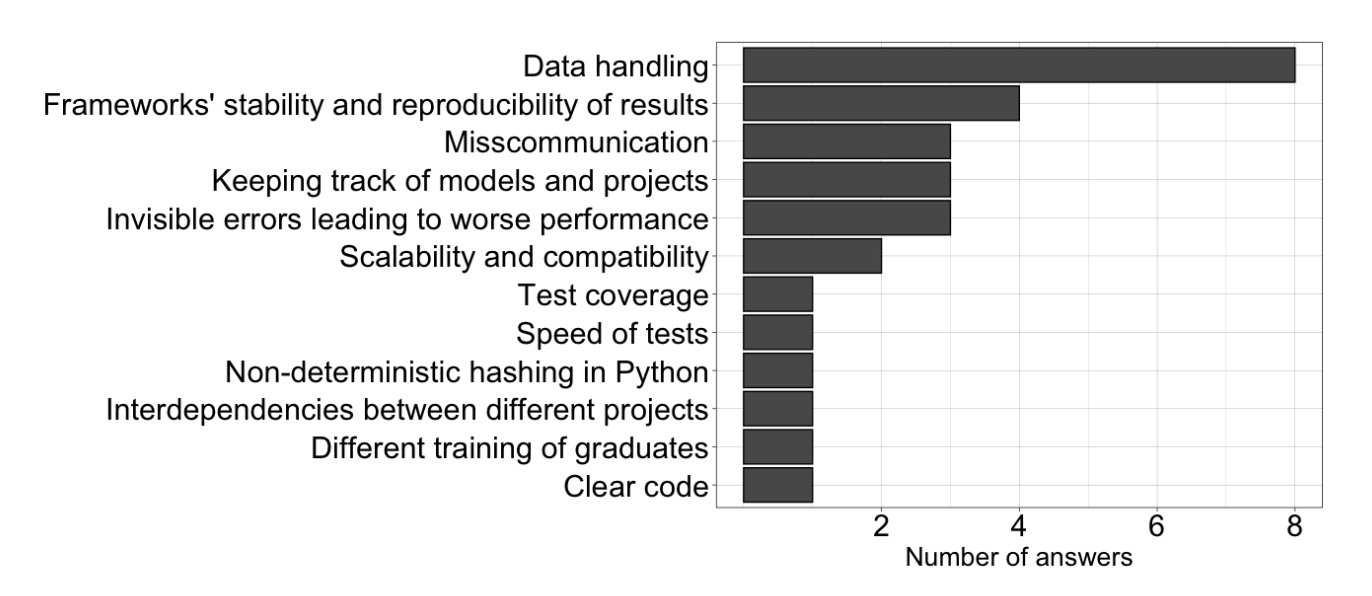
\includegraphics[width=0.8\textwidth]{issues.png}
    \caption{Issues in development of AI-enabled systems}
    \label{fig:issues}
\end{figure}

Figure \ref{fig:issues} illustrates the 12 issues identified by industry engineers in the development of AI-enabled systems and their frequency. The most common challenge, reported by 8 companies, is data handling issues. These issues encompass all stages of the data pipeline, including data collection, labeling, management, and preparation. As one interviewee noted, data-related problems are significant, with data preparation alone accounting for the largest proportion of effort (80\%). A poor dataset is difficult to manage and requires substantial time and effort. Another participant said: \textit{“I did not have that many problems with the code. Most of the time, when I am reading through the project, it is easy to read and understand. I mostly have problems with the data.”}

One potential application of BoundMiner in a large AI-intensive project is to test the dataset and identify types of data that need to be additionally collected. Data imbalance is a well-known issue in data analysis, and collecting data corresponding to the minority class is useful. However, it is not just the minority class that can make classification challenging. Data points that are similar to each other but have different labels can also lead to poor performance. BoundMiner could be particularly helpful in identifying edge test cases where the model struggles to make a decision. Collecting or synthetically generating more of this type of data could be beneficial in preparing and training the model.

In addition to summarizing the SQA challenges faced by practitioners, the authors also outlined the most commonly used practices for quality assurance of AI components. The most frequently mentioned practice is unit testing (mentioned by 8 companies). However, some interview participants noted that unit tests are not always the most effective method for quality assurance in AI-enabled systems. As one participant remarked: \textit{“I am personally not 100\% sure if unit testing in the machine learning field is very useful. A lot of data science guys follow one idea one week and the next idea next week. Unit tests which they wrote in week number one are completely useless for week number two because the approach is completely different.”} This observation highlights that AI-enabled software fundamentally differs from traditional software development, as data is the most critical aspect, while the code frequently changes. The current implementation of BoundMiner focuses on unit testing for traditional software. However, as previously mentioned, shifting the focus from code testing to dataset testing within BoundMiner appears to be more promising for AI-enabled projects. One potential challenge with dataset testing is the large size of inputs, such as images, which could lead BoundMiner to consume more resources in terms of memory and time. An input preprocessing step may need to be added to the Boundary Value Analysis process. We should also consider integrating an effective dimensionality reduction technique that preserves the key qualities of data inputs.

\end{document}